\section{Introducción}
El proyecto realizado responde en primera instancia a mi interés personal, pero a su vez, se puede plantear como el desarrollo de un producto. Este producto se enmarca en el sector de los componentes electrónicos de audio para uso profesional ya que pretende crear un tipo de dispositivo que no se utiliza hasta la fecha: pedales de efectos para instrumentos no electrófonos con funcionamiento en tiempo real. Este producto tiene un ciclo de vida amplio que parte desde el montaje de los componentes pasando por el ensamblaje y transporte hasta su uso particular para de reciclaje posterior. 

Actualmente existen en el mercado multitud de empresas que comercializan modelos de pedales de características similares íntimamente relacionadas con el desarrollo de nuevas tecnologías y componentes electrónicos que facilitan los avances en este campo. A su vez, con el acercamiento de la música a las clases populares que esta teniendo lugar en nuestros días, la cifra de potenciales clientes va aumentando significativamente con el tiempo.

Por ello, aunque no exite una necesidad real de un dispositivo de estas características, si existe un hueco en el mercado que podría verse resuelto con la adquisición de este o diseños similares por parte de alguna empresa de audio ya asentada.
\section{Descripción de impactos relevantes y análisis de los mismos}
Para la descripción de los diferentes impactos del desarrollo del proyecto, se incluye la figura \ref{fig:aspectos} siguiendo el modelo propuesto en la guía para la realización de este anexo proporcionada por la escuela.

De todos ellos, cabe destacar el impacto de los aspectos económicos, ya que resultan de especial relevancia en el desarrollo de un producto. En general, como cualquier proyecto basado en electrónico, llama la atención el bajo costo de los componentes, frente al elevado coste de ingeniería y montaje relacionado con el mismo. Así mismo, cabe destacar que el pedal está pensado para un uso continuado sin mantenimiento, lo que reduce el número de piezas necesarias para su correcto funcionamiento a lo largo de los años.

De cara a los aspectos medioambientales, es necesario tener en cuenta algunas predicciones relacionadas con la cantidad restante en la naturaleza de algunos elementos que que se utilizan en la fabricación de los componentes. Según estas, en algunas pocas décadas, el costo de extracción o refinamiento de algunos metales podría superar su valor en el mercado, provocando un encarecimiento de los precios o escasez de los mismo. En cualquier caso, para el desarrollo de este producto, orientado al corto-medio plazo, no debería haber ningún problema de este tipo. Es más, el uso de una FPGA favorece el reutilizamiento de los recursos hardware, por lo que se pueden llevar a cabo actualizaciones de versiones sin cambiar componentes, maximizando el aprovechamiento del producto.
 
\begin{figure}[!th]
\begin{center}
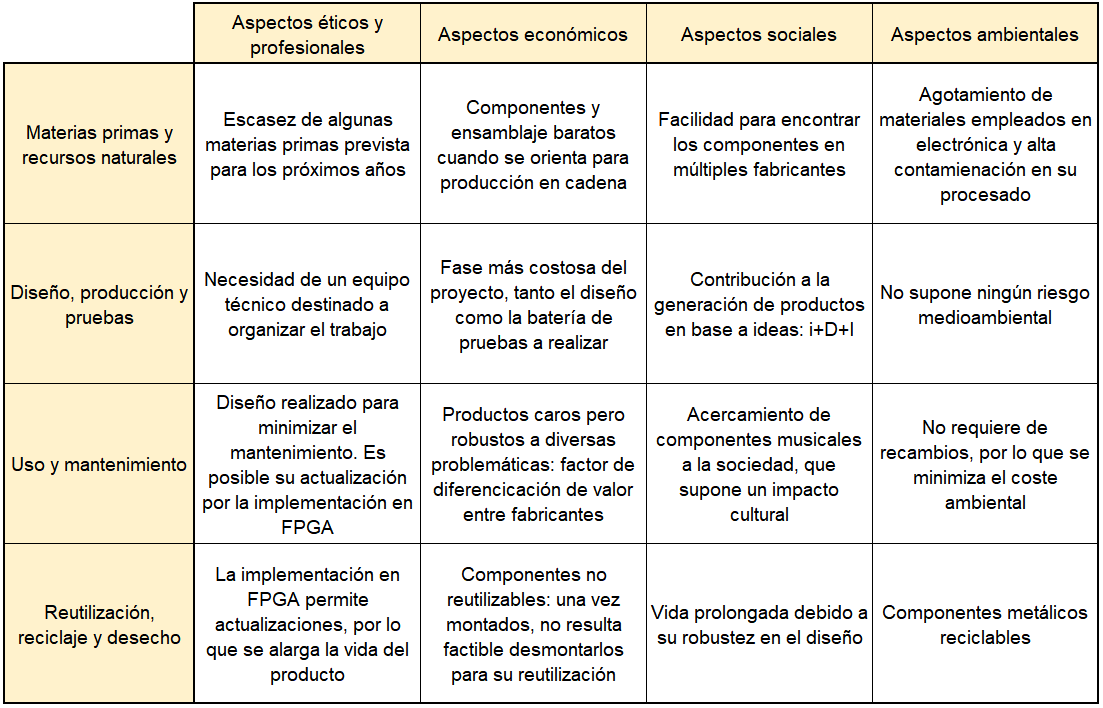
\includegraphics[width=14cm]{img/aspectos.png}
\caption{\label{fig:aspectos}Relación de los posibles impactos en diferentes ámbitos}
\end{center}
\end{figure}

Los aspectos sociales son, quizás, los menos relevantes ya que al producto esta orientado al mundo musical, que generalmente se trata como un elemento de ocio en la mayoría de los casos. El uso profesional está mucho más complicado debido al poco nivel de innovación que existe actualmente en cuanto a técnicas de producción.

\section{Conclusiones}
Tratándose de un proyecto planteado de forma personal, evidentemente no hay grandes impactos en el conjunto de la sociedad. No obstante, hay que destacar los aspectos económicos como los más relevantes. Al fin y al cabo, estos son los más importantes en cuanto a un producto comercial. Los bajos costos permiten rentabilizar en gran medida la inversión realizada en la fase de diseño, favoreciendo las ganancias totales a largo plazo.